
\newcommand{\Sswix}{
    \begin{figure}[t]
        \centering
        \lstinputlisting{figures/swift.scala}
        \caption{An example usage of the Swift Matrix Library.}
        \label{fig:swix}
    \end{figure}
}
\newcommand{\Sbudget}{
    \begin{figure}
        \centering
        \begin{tabular}{c | c}
            Item & Cost \\
            \hline
            Myo armbands            & \$318 \\
            Apple Developer License & \$100 \\
            Video production        & \$300 \\
        \end{tabular}
        \caption{Our project's budget.}
        \label{fig:budget}
    \end{figure}
}

\newcommand{\Stimeline}{
    \begin{figure}
        \centering
        \begin{tabular}{r |@{\foo} l}
            Completing math library & Sept -- Oct \\
            Making app work with armbands & Sept -- Nov \\
            Devising algorithm & Dec -- March \\
            Publishing results & March -- May\\
        \end{tabular}
        \caption{The proposed timeline.}
        \label{fig:timeline}
    \end{figure}
}
\newcommand{\Sscreenshot}{
    \begin{figure}
        \centering
        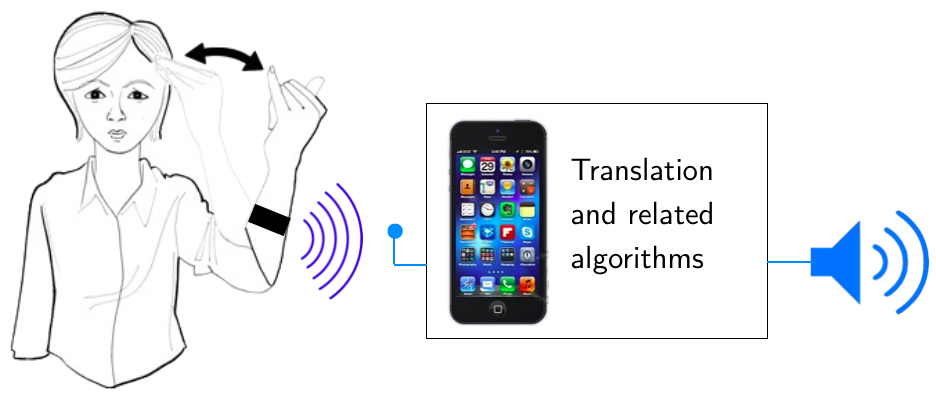
\includegraphics[width=0.4\textwidth]{figures/screenshot}
        \caption{A screenshot of an early beta version.}
        \label{fig:screenshot}
    \end{figure}
}
\newcommand{\Smyo}{
    \begin{figure}
        \centering
        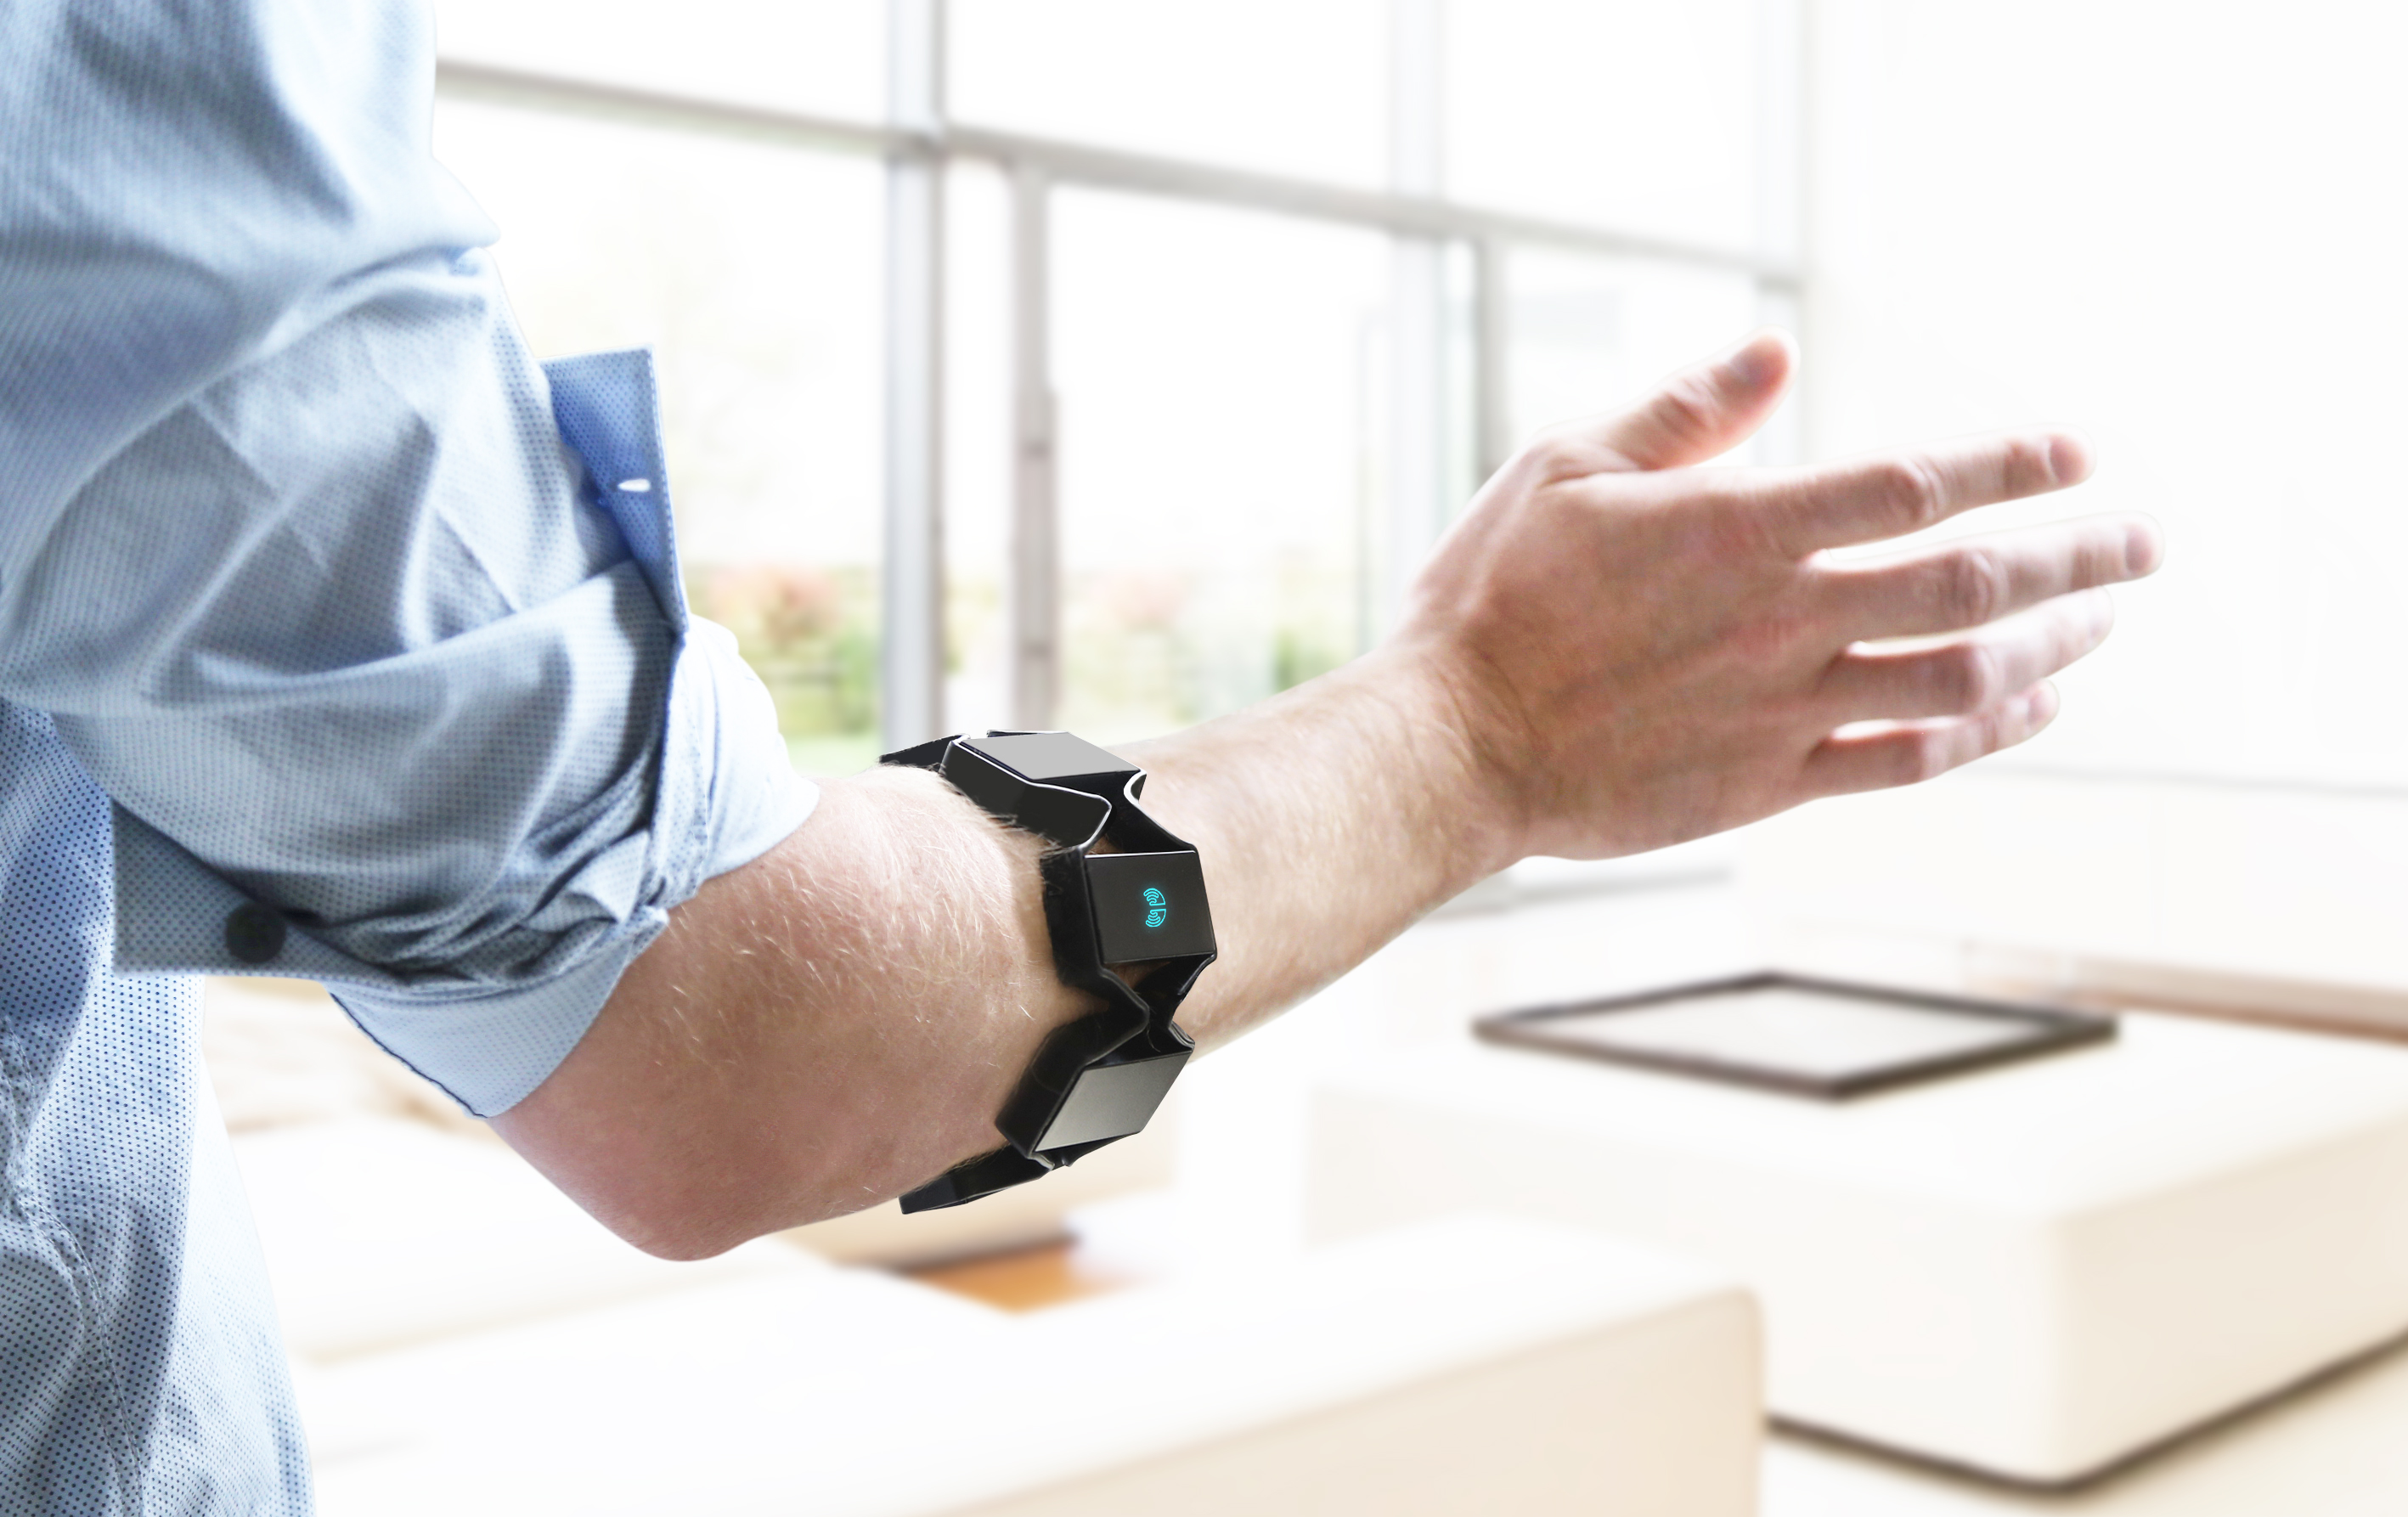
\includegraphics[width=0.4\textwidth]{figures/myo}
        \caption{The Myo armbands in use.}
        \label{fig:armbands}
    \end{figure}
}
\newcommand{\Stitlepic}{
    \begin{figure}[h]
        \centering
        \begin{tikzpicture}
        \begin{scope}
            \clip [rounded corners=.5cm] (0,0) rectangle coordinate (centerpoint) (4,4cm); 
            \node [inner sep=0pt] at (centerpoint) 
            {\includegraphics[width=4.0cm]{../../gesture/imgs/icon/icon}}; 
        \end{scope}
        \end{tikzpicture}
    \end{figure}
}

